\documentclass{beamer}

\usepackage{beamerthemesplit}
\usetheme{Singapore} 

\input{../../include/preamble.inc} 
\input{../../include/definitions.inc} 
\input{../../include/author.inc} 

\title[]{Элементы дифференциальной геометрии. Скалярные и векторные поля.}

\begin{document}

\frame{\titlepage}

\frame{
\frametitle{Аннотация}

\parbox{\textwidth}{
Кривая в пространстве. Ортогональная система координат, связанная с кривой. Формулы Френе. Скалярные и векторные поля. Поверхности уровня. Векторные линии.
}
}


\frame{
\frametitle{Система координат в $\Rd{3}$}
\parbox{\textwidth}{
Введем в векторном пространстве $\Rd{3}$ систему координат \pause и три базисных ортонормированных вектора $\basis{i}$, $\basis{j}$ и $\basis{k}$. 

}

\bigskip\bigskip
\begin{columns}
\begin{column}{0.3\textwidth}
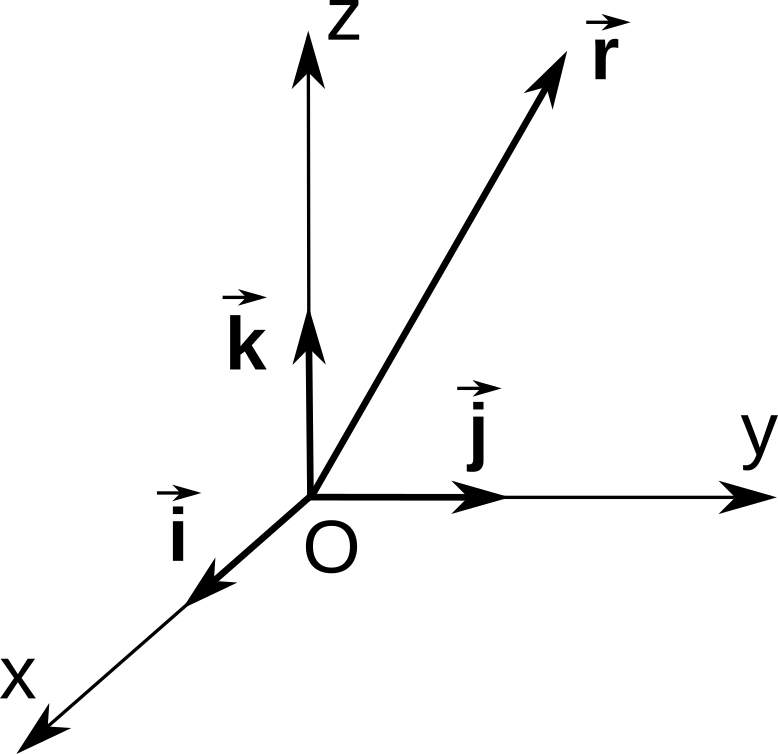
\includegraphics[width=\textwidth]{../img/axis.png} \pause 
\end{column}
\begin{column}{0.7\textwidth}
Тогда произвольный вектор $\vec{r}$ можно представить в виде:
\[
\vec{r}=x\basis{i}+y\basis{j}+z\basis{k},
\] \pause 
где $x$, $y$, $z$ -- координаты вектора $\vec{r}$ в указанном базисе.
\end{column}
\end{columns}



}

\frame{
\frametitle{Вектор, зависящий от параметра}


\parbox{\textwidth}{
В $\Rd{3}$ рассмотрим переменный вектор 
\[ 
\vec{a}(t)=a_x(t)\basis{i}+a_y(t)\basis{j}+a_z(t)\basis{k},\pause 
\]
где $a_x(t)$, $a_y(t)$, $a_z(t)$ -- декартовы координаты вектора, непрерывно зависящие от $t$.\pause 

}

\begin{columns}
\begin{column}{0.3\textwidth}
\centering
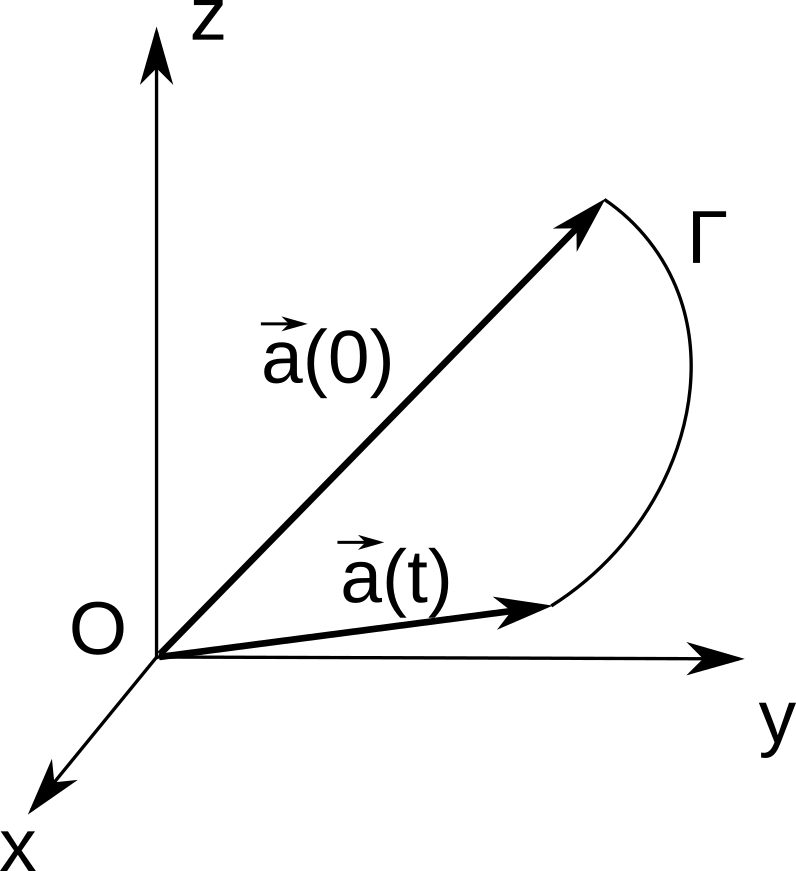
\includegraphics[width=\textwidth]{../img/godograf.png}\pause 
\end{column}
\begin{column}{0.7\textwidth}
\begin{dfn}
\parbox{\textwidth}{
Геометрическое место точек $\Gamma$ концов вектора $ \vec{a}(t) $, отложенных из общего начала $O$, называется \alert{годографом} вектора.
}
\end{dfn}
\end{column}
\end{columns}





}



\frame{
\frametitle{Производная вектора}

\begin{dfn}
\alert{Производной} векторной функции называется
\[ 
\vec{a}'(t)=\frac{d\vec{a}}{dt}=\lim_{\Delta t\rightarrow 0}\frac{\vec{a}(t+\Delta t)-\vec{a}(t)}{\Delta t}.
\]
\end{dfn}\pause 
\begin{columns}
\begin{column}{0.4\textwidth}
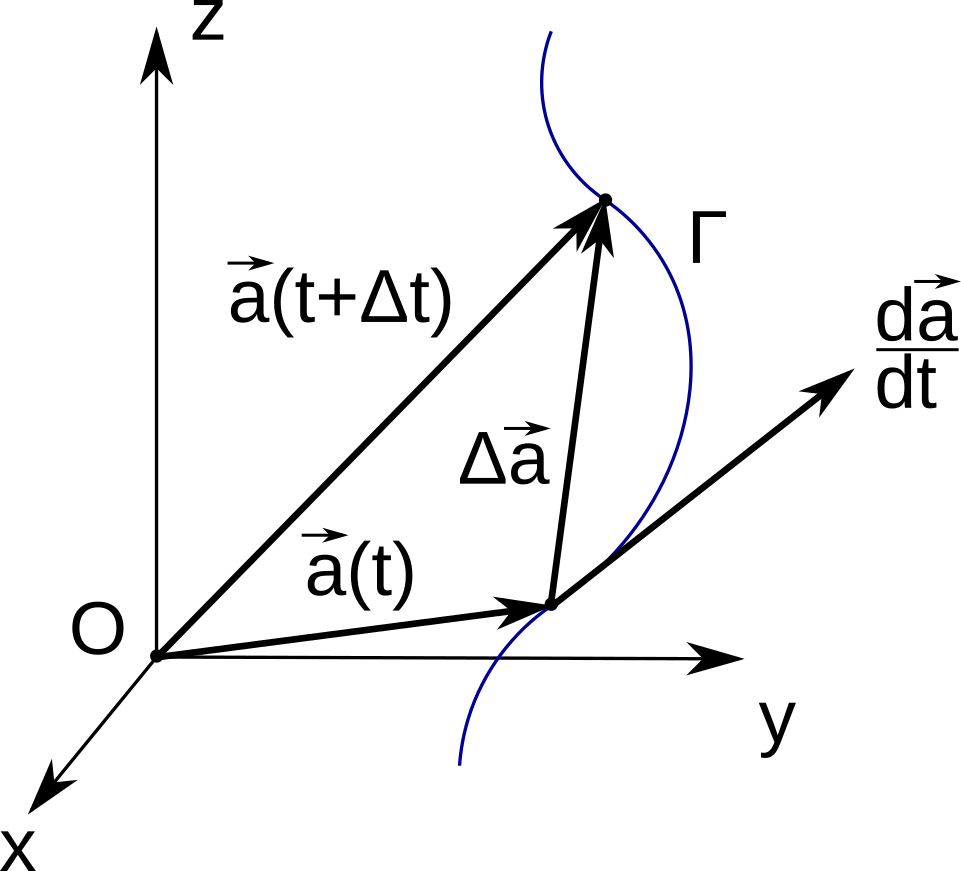
\includegraphics[width=\textwidth]{../img/derivative.png}
\end{column}\pause 
\begin{column}{0.6\textwidth}
\parbox{\textwidth}{
$ \dtds{\vec{a}} $ по направлению совпадает с касательной к годографу $\Gamma$ вектора $\vec{a}(t)$.

\bigskip
На рисунке 
$\Delta \vec{a} = \vec{a}(t+\Delta t)-\vec{a}(t)$.

}
\end{column}
\end{columns}
}
\frame{
\frametitle{Свойства производной вектора}
\scriptsize
\parbox{\textwidth}{
Пусть $\vec{a}(t)$, $\vec{b}(t)$ -- векторные функции; $c(t)$ -- скалярная функция; $\cdot$, $\times$ -- операции скалярного и векторного произведения, тогда \pause 
\begin{enumerate}
\item 
$\vec{a}'(t)= \pause 
\displaystyle\lim_{\Delta t\rightarrow 0}\displaystyle\frac{\vec{a}(t+\Delta t)-\vec{a}(t)}{\Delta t} = $ \pause 
\[
=\lim_{\Delta t\rightarrow 0}\left(
\frac{a_x(t+\Delta t)-a_x(t)}{\Delta t}\basis{i}+
\frac{a_y(t+\Delta t)-a_y(t)}{\Delta t}\basis{j}+
\frac{a_z(t+\Delta t)-a_z(t)}{\Delta t}\basis{k}
\right)=
\] \pause 
\[
=\dt{a_x}\basis{i}+\dt{a_y}\basis{j}+\dt{a_z}\basis{k};
\] \pause 
\item
$\dtds{(c\vec{a})}  =  \dtds{c}\vec{a}+c\dtds{\vec{a}}$; \pause 

\item
$\dtds{(\vec{a}\cdot\vec{b})} = \dtds{\vec{a}}\cdot\vec{b}+\vec{a}\cdot\dtds{\vec{b}}$; \pause 

\item
$\dtds{(\vec{a}\times\vec{b})}  =  \dtds{\vec{a}}\times\vec{b}+\vec{a}\times\dtds{\vec{b}}$. \pause 

\end{enumerate}
Справедливость выражений пунктов 2-4 следует из пункта 1. 
}
}


\frame{
\frametitle{Производная вектора постоянного направления}
\parbox{\textwidth}{
Пусть $\vec{a}(t)=a(t)\vec{a}_0$, где $||\vec{a}_0||=1$ -- постоянный вектор, $a(t)$ -- длина вектора $\vec{a}(t)$,  \pause тогда
\[
\dt{\vec{a}}=\dt{a}\vec{a}_0.
\] \pause 

\bigskip
Отсюда следует, что \alert{$\dtds{\vec{a}} || \vec{a}$}.
}

}

\frame{
\frametitle{Производная вектора постоянной длины}
\parbox{\textwidth}{
Пусть $\vec{a}(t)=a_0\vec{b}(t)$, где $a_0$ -- заданная длина, $||\vec{b}(t)||=1$ --  направление вектора $\vec{a}(t)$,  \pause тогда
\[
\dt{\vec{a}}=a_0\dt{\vec{b}}.
\] \pause 
Рассмотрим
\[
\dt{(\vec{a}\cdot\vec{a})}= \pause 
\dt{\vec{a}}\cdot\vec{a}+\vec{a}\cdot\dt{\vec{a}}= \pause 
2\vec{a}\cdot\dt{\vec{a}}.
\] \pause 
С другой стороны, 
\[
\dt{(\vec{a}\cdot\vec{a})}=\dt{a_0^2}=0.
\] \pause 
Отсюда следует, что $\vec{a}\cdot\dtds{\vec{a}} = 0$ или \alert{$\vec{a} \perp \dtds{\vec{a}}$}.

}

}

\frame{
\frametitle{Длина производной вектора единичной длины}


\begin{columns}
\begin{column}{0.3\textwidth}
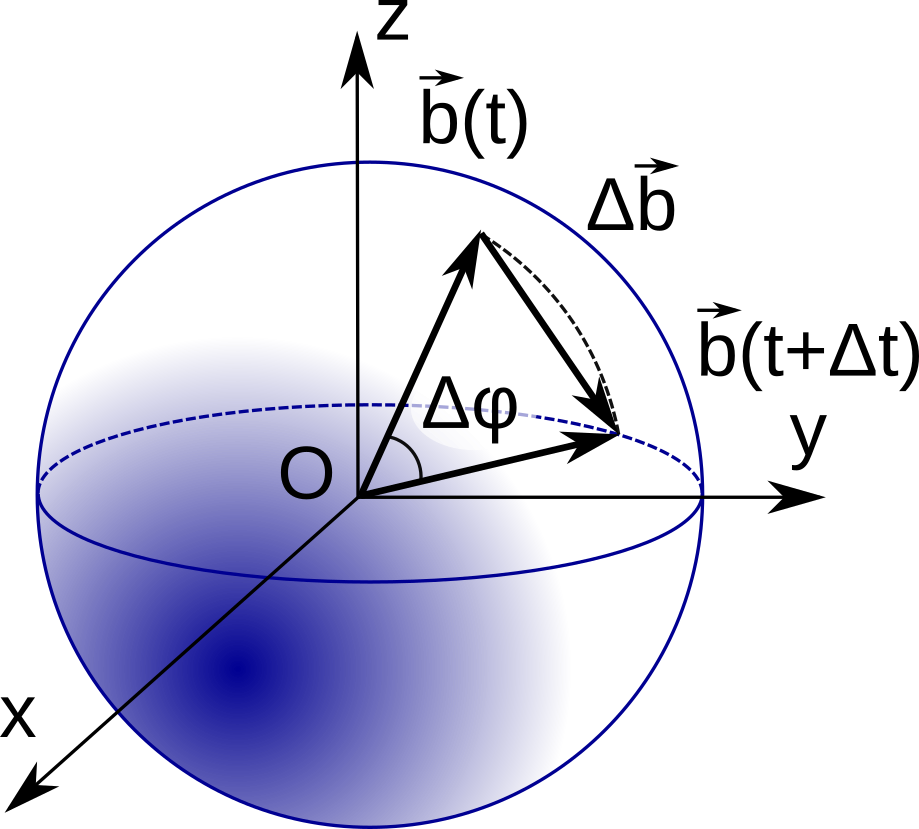
\includegraphics[width=\textwidth]{../img/angle_velocity.png}\\ \pause 
\end{column}
\begin{column}{0.7\textwidth}
\parbox{\textwidth}{

На рисунке: $\Delta\varphi$ -- угол между двумя положениями $\vec{b}$, 
\[
\Delta \vec{b} = \vec{b}(t+\Delta t)- \vec{b}(t), 
\]
\[
||\Delta \vec{b}|| = 2 \sin(\Delta\varphi/2).
\] \pause 
\[ 
\left|\left|\dt{\vec{b}}\right|\right|= \pause 
\lim_{\Delta t\rightarrow 0}\frac{||\Delta \vec{b}||}{\Delta t}= \pause 
\lim_{\Delta t\rightarrow 0}\frac{2\sin(\Delta\varphi/2)}{\Delta t}= \pause 
\]
\[
=\lim_{\Delta t\rightarrow 0}\frac{\Delta\varphi}{\Delta t}. \pause 
\]
$ \omega=\lim_{\Delta t\rightarrow 0}\frac{\Delta\varphi}{\Delta t}$ -- называется \alert{угловой скоростью}.
}
\end{column}
\end{columns}



}


\frame{
\frametitle{Параметризация кривой с помощью длины $s$}

\begin{columns}
\begin{column}{0.3\textwidth}
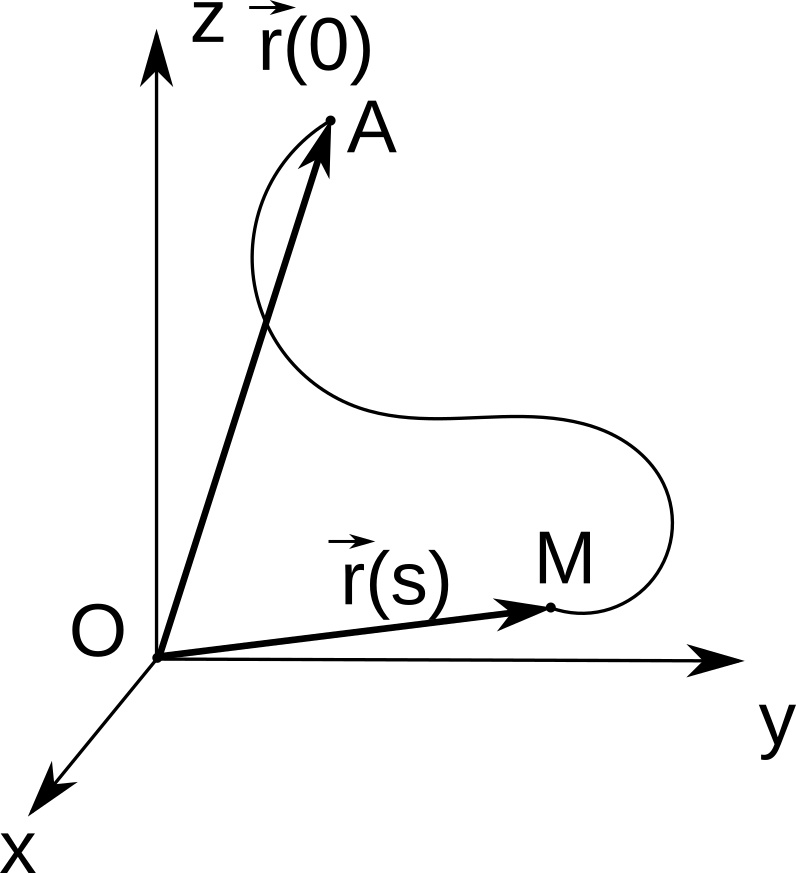
\includegraphics[width=\textwidth]{../img/curve_s.png}\\ \pause 
\end{column}
\begin{column}{0.7\textwidth}
\parbox{\textwidth}{
Пусть кривая параметризована с помощью расстояния $s$ от точки $A$  \pause и её уравнение задано некоторым радиус вектором 
\[
\vec{r}(s)=x(s)\basis{i}+y(s)\basis{j}+z(s)\basis{k}
\]
в некоторой декартовой системе координат, где $s$ -- длина дуги $AM$.
}
\end{column}
\end{columns}
}

\frame{
\frametitle{Вектор касательной к кривой}

\begin{columns}
\begin{column}{0.3\textwidth}
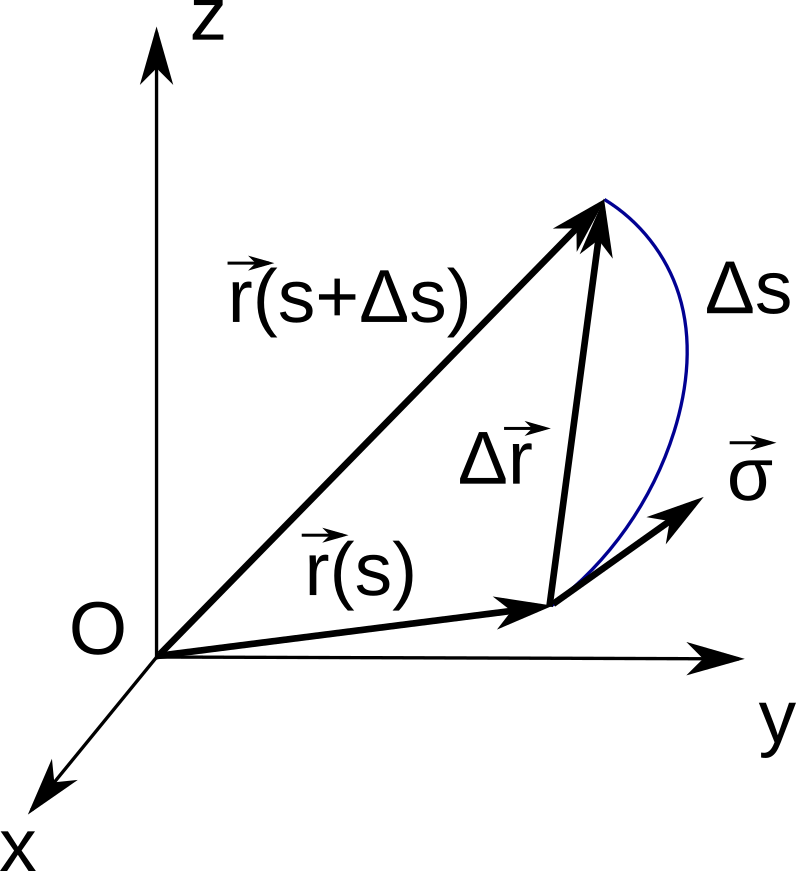
\includegraphics[width=\textwidth]{../img/tangent.png}\\ \pause 
\end{column}
\begin{column}{0.7\textwidth}
\parbox{\textwidth}{Вектор $ \ds{\vec{r}} $ направлен по касательной к рассматриваемой кривой,  \pause кроме того
\[ 
\left|\left|\ds{\vec{r}}\right|\right|=\lim_{\Delta s\rightarrow 0}\frac{||\Delta\vec{r}||}{\Delta s}=1.
\]  \pause 
Таким образом единичный вектор касательной к кривой 
\[ 
\vec{\sigma}=\ds{\vec{r}}=\sigma_x\basis{i}+\sigma_y\basis{j}+\sigma_z\basis{k}, \quad ||\vec{\sigma}||=1.
\] \pause 
Компоненты вектора $\vec{\sigma}$ по осям 
\[
\begin{array}{c}
\sigma_x = \ds{x} = cos(\vec{\sigma},x),\\
\sigma_y = \ds{y} = cos(\vec{\sigma},y),\\
\sigma_z = \ds{z} = cos(\vec{\sigma},z).
\end{array}
\]



}
\end{column}
\end{columns}

}

\frame{
\frametitle{Радиус кривизны}

\begin{columns}
\begin{column}{0.3\textwidth}
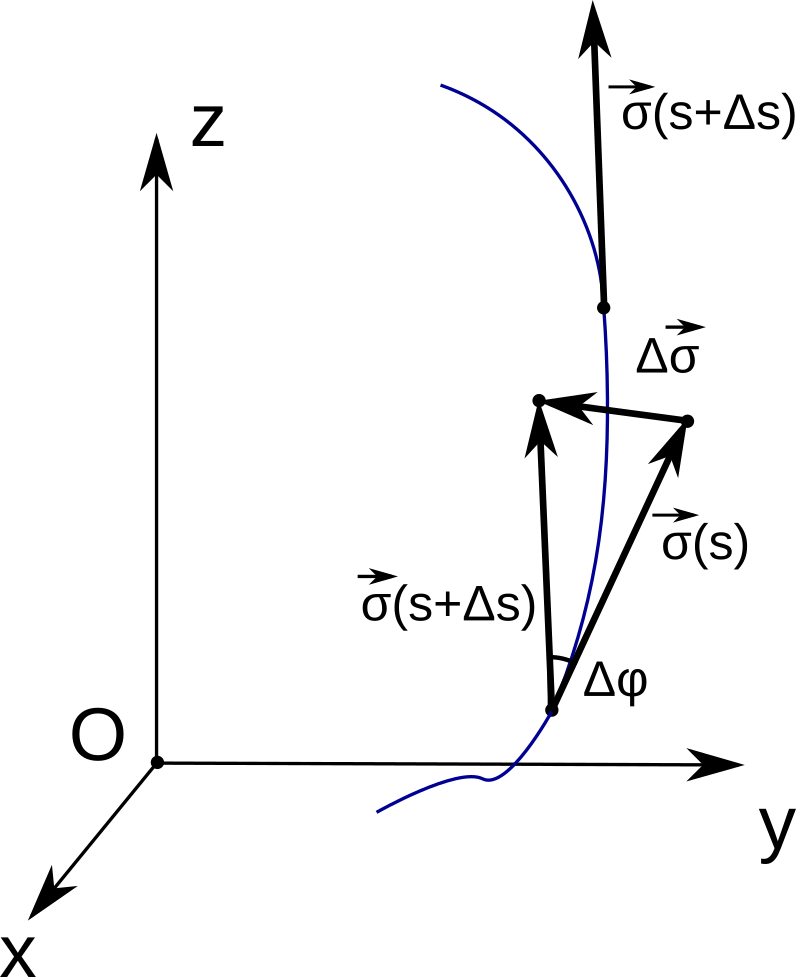
\includegraphics[width=\textwidth]{../img/curve_r_1.png}\\
\end{column} \pause 
\begin{column}{0.7\textwidth}

\parbox{\textwidth}{
Рассмотрим длину производной касательного вектора.  \pause Так как $||\vec{\sigma}(s)||=1$, тогда справедливо
\[ 
\left|\left|\dsd{\vec{r}}\right|\right|= \pause 
\left|\left|\ds{\vec{\sigma}}\right|\right|= \pause 
\lim_{\Delta s\rightarrow 0}\frac{\Delta\varphi}{\Delta s}= \pause 
\frac{1}{R(s)}.
\]

}

\end{column}
\end{columns} \pause 

\begin{dfn}
\parbox{\textwidth}{
Величина $R(s)$, определяемая формулой, называется \alert{радиусом кривизны} кривой.
}
\end{dfn} \pause 

\medskip
Радиус кривизны кривой определяется соотношением
\[ 
R(s)=1/\sqrt{\left(\dsd{x}\right)^2+\left(\dsd{y}\right)^2+\left(\dsd{z}\right)^2}.
\]

}

\frame{
\frametitle{Соприкасающаяся плоскость}
\begin{dfn}
\parbox{\textwidth}{
\alert{Соприкасающая плоскость} --  плоскость, в которой лежит данная точка и вектора $\ds{\vec{\sigma}}$ и $\vec{\sigma}$. \pause 
}
\end{dfn}
\begin{columns}
\begin{column}{0.3\textwidth}
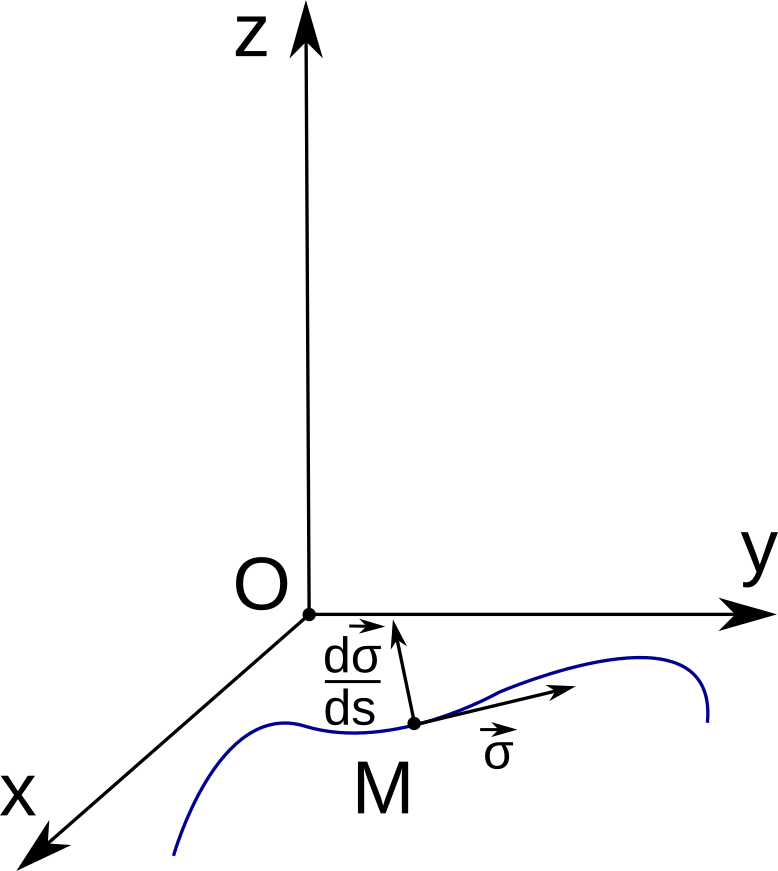
\includegraphics[width=\textwidth]{../img/planes.png} \pause 
\end{column}
\begin{column}{0.7\textwidth}

\parbox{\textwidth}{
На рисунке кривая лежит в плоскости $Oxy$, следовательно касательная и её производная тоже лежат в этой плоскости. Поэтому $Oxy$ является \alert{соприкасающейся плоскостью}.
}




\end{column}
\end{columns}


}

\frame{
\frametitle{Вектор нормали к кривой}

\begin{columns}
\begin{column}{0.3\textwidth}
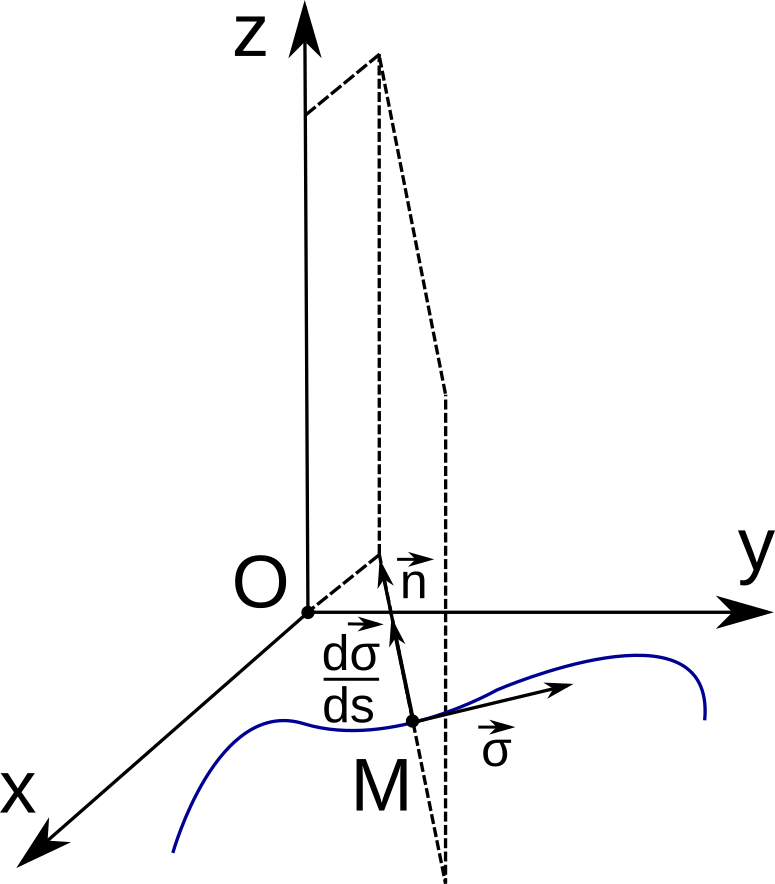
\includegraphics[width=\textwidth]{../img/normal.png} \pause 
\end{column}
\begin{column}{0.7\textwidth}

\parbox{\textwidth}{
\begin{dfn}
\parbox{\textwidth}{
Прямые, перпендикулярные касательной, называются \alert{нормалями} к кривой, а плоскость, их содержащая -- \alert{нормальной плоскостью} к кривой в данной точке. 
}
\end{dfn} \pause 

\begin{dfn}
\parbox{\textwidth}{
Нормаль, лежащая в соприкасающейся плоскости, называется \alert{главной нормалью}.
}
\end{dfn} \pause 

Т.к вектор $ \ds{\vec{\sigma}} \perp \vec{\sigma}$ и лежит в соприкасающей плоскости,  \pause то
\[ 
\dsd{\vec{r}}=\ds{\vec{\sigma}}=\frac{\vec{n}}{R},
\] \pause 
$ \vec{n} $ -- единичный вектор, направленный в сторону главной нормали.
}
\end{column}
\end{columns}
}


\frame{
\frametitle{Вектор бинормали}



\begin{columns}
\begin{column}{0.3\textwidth}
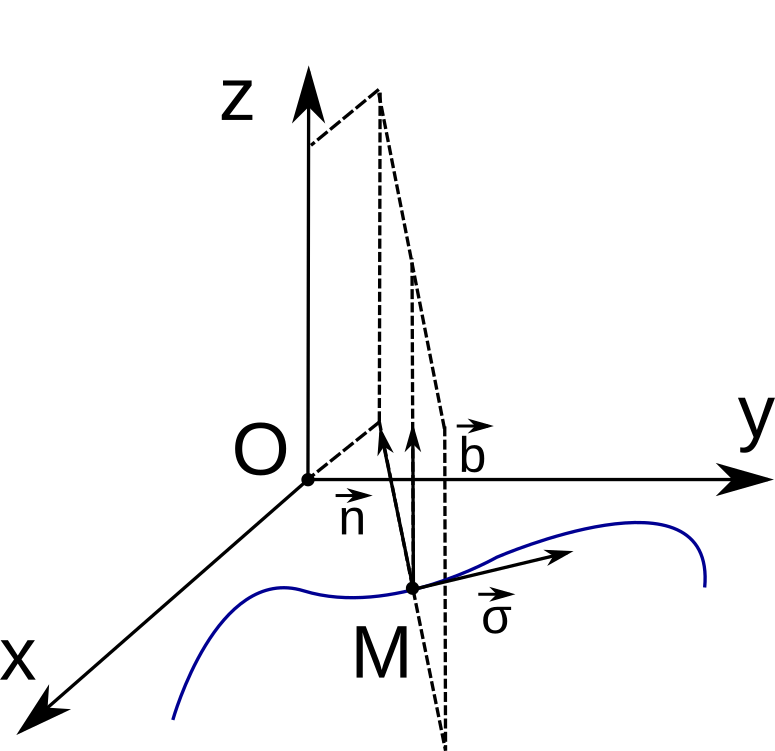
\includegraphics[width=\textwidth]{../img/binormal.png} \pause 
\end{column}
\begin{column}{0.7\textwidth}
\begin{dfn}
\parbox{\textwidth}{
Нормаль к кривой, перпендикулярная к соприкасающейся плоскости, называется \alert{бинормалью}. \pause 
В качестве бинормали будем подразумевать вектор
\alert{\[ 
\vec{b}=\vec{\sigma}\times\vec{n}.
\]}
}
\end{dfn}
\end{column}
\end{columns}


}

\frame{
	\frametitle{ Производная от бинормали }
	

	\parbox{\textwidth}{
		Рассмотрим
		$\dsds{\vec{b}}= \pause 
		\ds{(\vec{\sigma}\times\vec{n})}= \pause 
		\ds{\vec{\sigma}}\times\vec{n} + \vec{\sigma}\times\ds{\vec{n}}.
		$
		\pause 
		\begin{itemize}
			
			\item $\dsds{\vec{\sigma}}\times\vec{n}= \pause 
			\displaystyle\frac{\vec{n}}{R}\times\vec{n}= \pause 0$ в силу коллинеарности $\vec{n} || \vec{n}$; \pause 
			
			\item $\dsds{\vec{b}} = \vec{\sigma}\times\dsds{\vec{n}}  \perp \vec{\sigma}$  \pause и, так как $||\vec{b}||=1$, то $\dsds{\vec{b}} \perp \vec{b}$, \pause поэтому
			\alert{ 
				\[
					\vec{\sigma}\times\dsds{\vec{n}} || \vec{n}.
				\]
				} \pause 
			
		\end{itemize}
		
		\vspace{-5pt}	
		\begin{exampleblock}{Связь бинормали и нормали}
			\parbox{\textwidth}{
				\[
				\dsds{\vec{b}} = -\frac{\vec{n}}{T(s)},
				\] 
				где $1/T$ называется кручением, $ T $ -- радиус кручения. Кручение~-- мера отклонения от плоской кривой.
			}
		\end{exampleblock}
%		В силу того, что $||\vec{b}||=1$, то
		
	}
}


\frame{
\frametitle{Производная от нормали}
\begin{columns}
\begin{column}{0.3\textwidth}
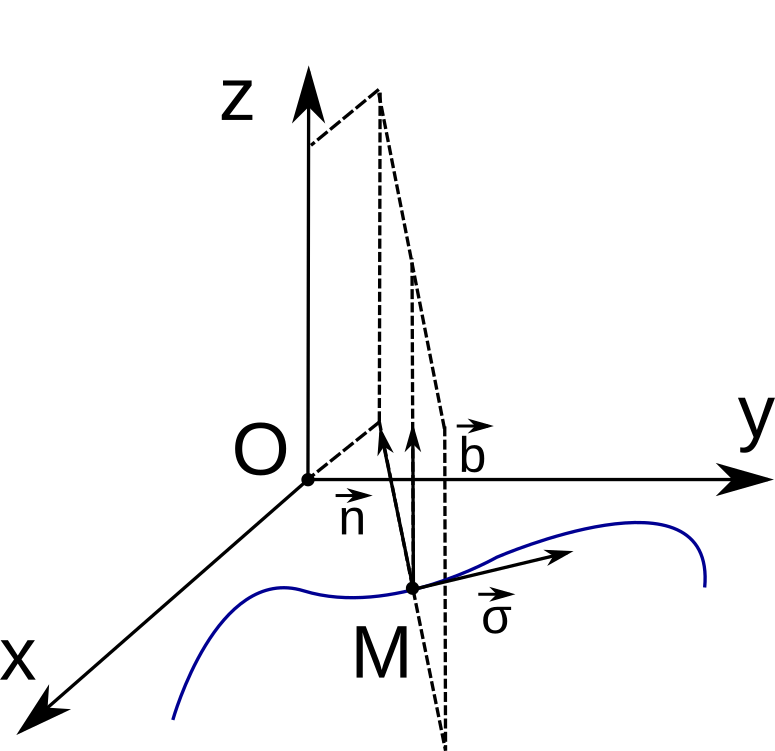
\includegraphics[width=\textwidth]{../img/binormal.png} \pause 
\end{column}
\begin{column}{0.7\textwidth}
\parbox{\textwidth}{
Т.к. вектора $\vec{\sigma}$, $\vec{n}$ и $\vec{b}$ составляют правую тройку ортонормированных векторов,  \pause то
\alert{\[
\vec{n}=\vec{b}\times\vec{\sigma}.
\]} \pause 
}
\end{column}
\end{columns}

\bigskip
Рассмотрим
\[
\ds{\vec{n}}= \pause 
\ds{\vec{b}}\times\vec{\sigma}+\vec{b}\times\ds{\vec{\sigma}}= \pause 
-\frac{\vec{n}}{T(s)}\times\vec{\sigma}+
\vec{b}\times\frac{\vec{n}}{R(s)}= \pause 
\frac{\vec{b}}{T(s)}-\frac{\vec{\sigma}}{R(s)}.
\]


}

\frame{
\frametitle{Формулы Френе}

\begin{dfn}
\parbox{\textwidth}{
Соотношения
\[ 
\ds{\vec{n}}=\frac{\vec{b}}{T(s)}-\frac{\vec{\sigma}}{R(s)}, \quad \ds{\vec{b}}=-\frac{\vec{n}}{T(s)}, \quad \ds{\vec{\sigma}}=\frac{\vec{n}}{R(s)},
\]
где $R(s)$, $T(s)$ -- радиусы кривизны и кручения кривой; $\vec{\sigma}$, $\vec{n}$ и $\vec{b}$ -- единичные касательный вектор, вектор главной нормали и бинормали, называются \alert{формулами Френе}.
}
\end{dfn}
}


\frame{
\frametitle{Скалярное и векторное поле}

\begin{dfn}
\parbox{\textwidth}{
Если в каждой точке пространства задана скалярная или векторная величина, то это означает, что задано \alert{скалярное} или \alert{векторное поле}.  \pause Если поле зависит от времени, то говорят о \alert{нестационарном поле}.
}
\end{dfn} \pause 


\begin{dfn}
\parbox{\textwidth}{
\alert{Поверхностью уровня} или \alert{изоповерхностью} называется поверхность, на которой скалярная величина остаётся постоянной.
}
\end{dfn} 

}

\frame{
\frametitle{}

\begin{dfn}
\parbox{\textwidth}{
Линия в векторном поле $ \vec{a}(\vec{r}) $, для которой в каждой точке вектор $\vec{a}$  её касается, называется \alert{векторной линией}.
}
\end{dfn} \pause 

\parbox{\textwidth}{
Пусть $\vec{r}(s)=x(s)\basis{i}+y(s)\basis{j}+z(s)\basis{k}$ -- векторная линия.  \pause По определению вектор касательной $\vec{\sigma}=\dsds{\vec{r}}$ параллелен вектору $\vec{a}(\vec{r})$  во всех точках области определения $s$,  \pause следовательно
\[
\begin{array}{c}
\dsds{x}=k a_x(x,y,z),\\
\dsds{y}=k a_y(x,y,z),\\
\dsds{z}=k a_z(x,y,z).
\end{array}
\] \pause 

Или, по-другому,
\[
\frac{dx}{a_x(x,y,z)}=\frac{dy}{a_y(x,y,z)}=\frac{dz}{a_z(x,y,z)}.
\]

}

}



\frame{
\frametitle{Поле температуры и ветра в Антарктиде 20.03.2016}
\centering
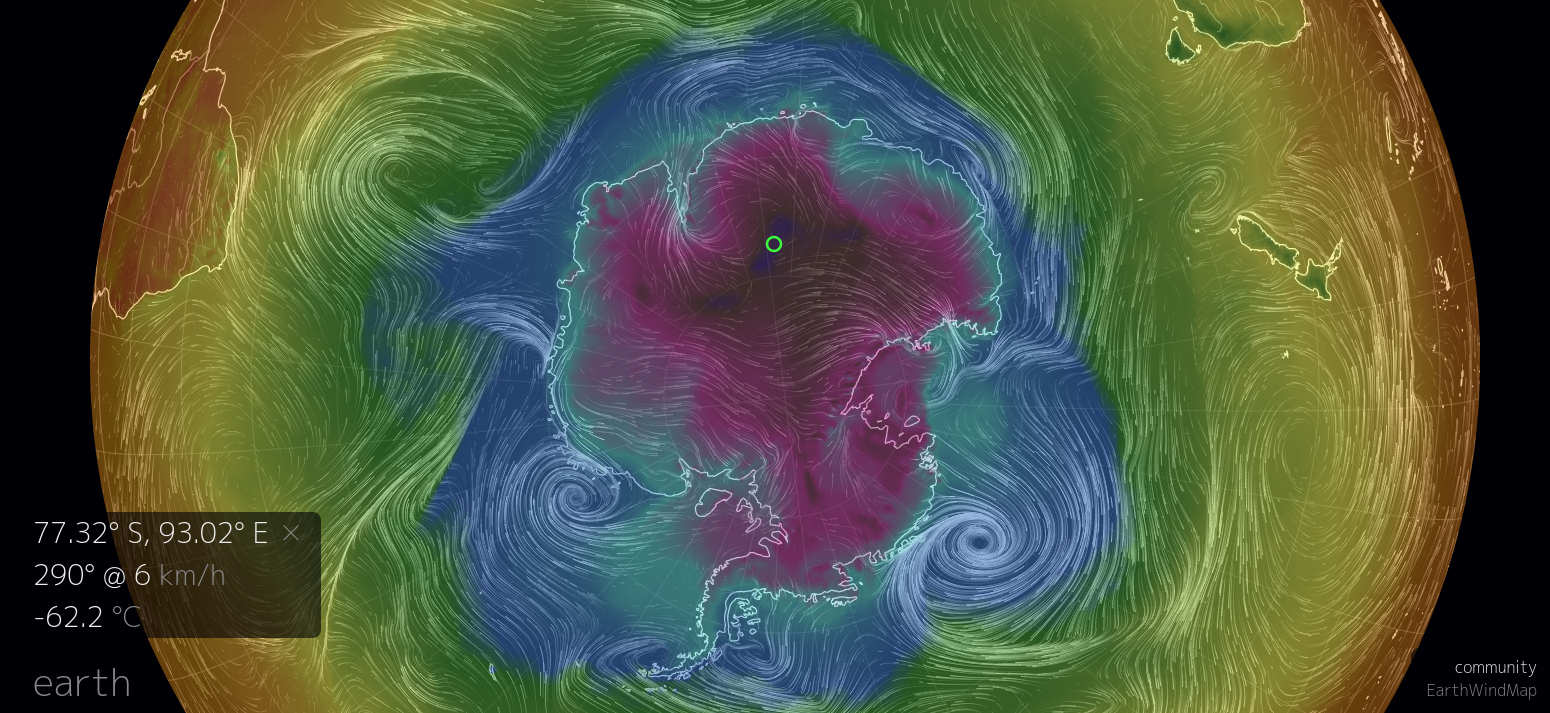
\includegraphics[width=\textwidth]{../img/earth.png}

\bigskip
\scriptsize
http://earth.nullschool.net/
}

\end{document}


